% =====================================================================
%  First World Model --- Apresentação (Beamer)
%  VQ-VAE + GPT Dynamics para CarRacing-v3
%  Compilar com pdflatex (compatível com Overleaf).
%  As imagens usam caminhos relativos a esta pasta (results/).
% =====================================================================
\documentclass[11pt,aspectratio=169]{beamer}

\usepackage[utf8]{inputenc}
\usepackage[T1]{fontenc}
\usepackage[brazil]{babel}
\usepackage{booktabs}
\usepackage{graphicx}
\usepackage{amsmath}
\usepackage{animate}   % anima frames (toca no Adobe Acrobat/Reader ou pdfpc)
\usepackage{tikz}
\usetikzlibrary{arrows.meta, positioning, shapes.geometric}

% ---- Tema / cores -------------------------------------------------
\usetheme{Madrid}
\usecolortheme{whale}
\useinnertheme{circles}
\setbeamertemplate{navigation symbols}{}
\setbeamertemplate{caption}{\raggedright\insertcaption\par}
\setbeamerfont{title}{size=\LARGE,series=\bfseries}
\setbeamercovered{transparent}

% Caminhos das imagens (relativos a results/)
\graphicspath{{./}{dreams/}{VQVAE/}}

% Cores de destaque
\definecolor{acc}{RGB}{46,139,87}      % verde pista/gramado
\definecolor{acc2}{RGB}{31,73,125}     % azul
\setbeamercolor{block title}{bg=acc2,fg=white}
\setbeamercolor{block body}{bg=acc2!8}

% ---- Metadados ----------------------------------------------------
\title[Mundos Imaginados]{Mundos Imaginados}
\subtitle{Aprendendo a Dinâmica do \texttt{CarRacing} com Tokens Visuais e um GPT Causal}
\author{Lucas Barcelos}
\institute{Relatório Técnico Parcial}
\date{\today}

% Atalho para nós do diagrama
\tikzset{
  stg/.style={rectangle, rounded corners, draw=acc2, thick, fill=acc2!10,
              text width=3.4cm, align=center, minimum height=0.95cm, font=\small},
  ar/.style={-{Stealth[length=3mm]}, thick, draw=acc2},
  % bloco de feature-map (largura ~ resolução, altura fixa)
  fmap/.style={rectangle, draw=acc2, thick, fill=acc!18, minimum height=1.6cm,
               font=\scriptsize, align=center},
  % célula de codebook
  cb/.style={rectangle, draw=acc2, thick, minimum width=0.42cm, minimum height=0.42cm,
             inner sep=0pt},
  op/.style={circle, draw=acc2, thick, fill=white, inner sep=1pt, font=\scriptsize},
  lbl/.style={font=\scriptsize\itshape, text=gray!60!black}
}

\begin{document}

% =====================================================================
\begin{frame}[plain]
  \titlepage
  \begin{center}
    \footnotesize\textcolor{gray}{Baseado em ``World Models'' (Ha \& Schmidhuber, 2018)}
  \end{center}
\end{frame}

% =====================================================================
\begin{frame}{Roteiro}
  \tableofcontents
\end{frame}

% =====================================================================
\section{Visão Geral}

\begin{frame}{Visão Geral}
  \textbf{Objetivo:} aprender um \emph{world model} do ambiente
  \texttt{CarRacing-v3} --- um modelo que simula (``sonha'') o próximo frame
  do jogo condicionado à ação do agente.

  \bigskip
  \begin{block}{Abordagem em dois estágios}
    \begin{enumerate}
      \item \textbf{Encoder perceptivo discreto} (VQ-VAE): comprime cada frame
            em um conjunto de \emph{tokens visuais}.
      \item \textbf{Modelo de dinâmica autorregressivo} (GPT causal): prevê a
            sequência de tokens do próximo frame dado o contexto e a ação.
    \end{enumerate}
  \end{block}

  \bigskip
  \small
  Discretizar a imagem transforma a previsão de frames em um problema de
  \textbf{modelagem de linguagem} --- trocamos regressão contínua por
  \emph{cross-entropy} sobre tokens.
\end{frame}

% =====================================================================
\begin{frame}{Pipeline Completo}
  \centering
  \begin{tikzpicture}[node distance=0.55cm]
    \node[stg] (env)  {Ambiente\\\texttt{CarRacing-v3}};
    \node[stg, below=of env] (ppo)  {Agente PPO\\(coleta de episódios)};
    \node[stg, below=of ppo] (vqvae){VQ-VAE Encoder\\$64{\times}64 \to 8{\times}8$};
    \node[stg, below=of vqvae] (gpt) {GPT Dynamics\\contexto de 19 frames};
    \node[stg, below=of gpt] (dream){Inferência / ``Sonho''};

    \draw[ar] (env)   -- node[right,font=\scriptsize]{frames $64{\times}64$ RGB} (ppo);
    \draw[ar] (ppo)   -- node[right,font=\scriptsize]{episódios \texttt{.npz}} (vqvae);
    \draw[ar] (vqvae) -- node[right,font=\scriptsize]{64 tokens/frame (codebook 512)} (gpt);
    \draw[ar] (gpt)   -- node[right,font=\scriptsize]{prevê frame $t{+}1$} (dream);
  \end{tikzpicture}
\end{frame}

% =====================================================================
\section{Coleta de Dados}

\begin{frame}{Coleta de Dados --- Agente PPO}
  \small\texttt{agente\_coleta/coleta.py}
  \medskip

  \begin{columns}[T]
    \begin{column}{0.55\textwidth}
      Um agente \textbf{PPO} pré-treinado (Stable-Baselines3) joga o
      \texttt{CarRacing-v3} com \textbf{5 ações discretas}
      (esquerda, direita, acelerar, frear, neutro).

      \medskip
      Para cobrir estados raros, aplica-se um cronograma de exploração
      \textbf{$\varepsilon$-greedy crescente}: a maior parte do dataset é de
      alta qualidade, mas uma fração introduz diversidade.
    \end{column}
    \begin{column}{0.42\textwidth}
      \centering
      \begin{table}
        \footnotesize
        \begin{tabular}{cc}
          \toprule
          $\varepsilon$ & Fração \\
          \midrule
          0.02 & 25\,\% \\
          0.05 & 25\,\% \\
          0.10 & 20\,\% \\
          0.20 & 15\,\% \\
          0.35 & 10\,\% \\
          0.60 &  5\,\% \\
          \bottomrule
        \end{tabular}
      \end{table}
      {\footnotesize Cronograma de exploração}
    \end{column}
  \end{columns}
\end{frame}

\begin{frame}{Coleta de Dados --- Pré-processamento}
  Cada episódio passa por um \emph{wrapper stack} antes de ser salvo:
  \medskip
  \begin{itemize}
    \item \texttt{FrameSkip(4)} --- acumula recompensa em 4 frames; reduz
          correlação temporal.
    \item \texttt{CropBlackBar(12)} --- remove a barra de informações inferior.
    \item \texttt{ResizeObservation($64{\times}64$)} --- redimensiona o frame.
    \item \texttt{NormalizeAndTranspose} --- $(H,W,C)$ uint8 $\to$ $(C,H,W)$
          float32 em $[0,1]$.
    \item \texttt{FrameStackChannels(4)} --- empilha 4 frames no eixo de canais
          (entrada do PPO).
  \end{itemize}

  \bigskip
  \begin{block}{Formato de saída}
    Cada episódio $\to$ \texttt{.npz} com
    \texttt{obs}$(T,3,64,64)$, \texttt{actions}$(T,)$,
    \texttt{rewards}$(T,)$ e \texttt{dones}$(T,)$.
  \end{block}
\end{frame}

% =====================================================================
\section{Encoder --- VQ-VAE}

\begin{frame}{Encoder --- VQ-VAE}
  \small\texttt{models/encoder/modules.py}, \texttt{models/encoder/train.py}
  \medskip

  Comprime cada frame $64{\times}64{\times}3$ em uma grade
  $8{\times}8 = \mathbf{64}$ \textbf{tokens discretos}, índices num
  \textbf{codebook de 512} entradas.

  \bigskip
  \begin{columns}[T]
    \begin{column}{0.5\textwidth}
      \textbf{Encoder} ($64{\times}64 \to 8{\times}8$)
      \begin{itemize}\small
        \item Conv $3{\times}3$ $\to$ 64 canais
        \item 4 estágios, \texttt{ch\_mult}=$[1,2,4,4]$, 2 ResnetBlocks cada
        \item Atenção espacial em $16{\times}16$ e $8{\times}8$
        \item 3 Downsamples $\to$ \texttt{latent\_dim}=256
      \end{itemize}
    \end{column}
    \begin{column}{0.5\textwidth}
      \textbf{Quantização Vetorial}
      \begin{itemize}\small
        \item Codebook $512 \times 256$
        \item Similaridade de cosseno
        \item EMA decay $=0.99$
        \item \emph{commitment weight} $=0.25$
      \end{itemize}
      \medskip
      \textbf{Decoder} ($8{\times}8 \to 64{\times}64$)
      \begin{itemize}\small
        \item Simétrico, \texttt{ch\_mult}=$[4,4,2,1]$
        \item Upsample (nearest + conv)
      \end{itemize}
    \end{column}
  \end{columns}
\end{frame}

\begin{frame}{VQ-VAE --- Arquitetura (diagrama)}
  \centering
  \resizebox{0.94\textwidth}{!}{%
  \begin{tikzpicture}[x=1cm,y=1cm]
    % ---- ENCODER: feature maps encolhem, canais crescem ----
    \node[fmap, minimum width=2.0cm] (e0) at (0,0)   {$64{\times}64$\\\textbf{3}};
    \node[fmap, minimum width=1.7cm] (e1) at (2.6,0) {$64{\times}64$\\\textbf{64}};
    \node[fmap, minimum width=1.4cm] (e2) at (4.9,0) {$32{\times}32$\\\textbf{128}};
    \node[fmap, minimum width=1.1cm] (e3) at (6.9,0) {$16{\times}16$\\\textbf{256}};
    \node[fmap, minimum width=0.8cm] (e4) at (8.6,0) {$8{\times}8$\\\textbf{256}};

    \draw[ar] (e0)--(e1); \draw[ar] (e1)--(e2); \draw[ar] (e2)--(e3); \draw[ar] (e3)--(e4);
    \node[lbl] at (2.6,-1.15) {conv\,in};
    \node[lbl] at (3.75,0.35) {$\downarrow2$};
    \node[lbl] at (5.9,0.35)  {$\downarrow2$};
    \node[lbl] at (7.75,0.35) {$\downarrow2$};
    \node[lbl, text=acc2] at (6.9,1.15) {attn};
    \node[lbl, text=acc2] at (8.6,1.15) {attn};

    % conv_out -> latente 256d @ 8x8
    \node[fmap, minimum width=0.8cm, fill=acc2!15] (z) at (10.6,0) {$8{\times}8$\\\textbf{256}\\\scriptsize latente};
    \draw[ar] (e4)--(z);

    % ---- tokens 8x8 (à direita) ----
    \node[fmap, minimum width=0.9cm, fill=acc!30] (tok) at (13.3,0) {$8{\times}8$\\\textbf{64 tokens}\\\scriptsize índices $\in[0,512)$};

    % ---- CODEBOOK (abaixo, entre latente e tokens) ----
    \node[draw=acc2, thick, rounded corners, fill=white, align=center, font=\scriptsize]
      (cbk) at (11.9,-1.9) {Codebook\\$512\times256$\\\scriptsize cosseno \textperiodcentered{} EMA};
    \draw[ar] (z) to[out=-90,in=180] node[lbl,below left,pos=0.9]{vizinho} (cbk);
    \draw[ar] (cbk) to[out=90,in=-90] (tok);

    % ---- DECODER (linha inferior, espelhado) ----
    \node[fmap, minimum width=0.9cm] (dz) at (13.3,-3.6) {$8{\times}8$\\\textbf{256}};
    \node[fmap, minimum width=2.0cm, fill=acc2!12] (dout) at (9.4,-3.6) {$64{\times}64$\\\textbf{3}\\\scriptsize frame};
    \draw[ar] (tok) -- node[lbl,right]{$z_q$} (dz);
    \draw[ar] (dz) -- node[lbl,below]{upsample $\times3$} (dout);

    % rótulos de grupo
    \node[font=\small\bfseries, text=acc2] at (5.5,1.9) {Encoder};
    \node[font=\small\bfseries, text=acc2] at (11.3,-2.9) {Decoder};
  \end{tikzpicture}}

  \smallskip
  {\footnotesize Cada frame $\to$ grade $8{\times}8$ de \textbf{64 tokens}; resolução cai
  $4\times$ e a profundidade sobe. Atenção só em $16{\times}16$ e $8{\times}8$.}
\end{frame}

\begin{frame}{Quantização Vetorial --- Mecanismo}
  \begin{columns}[c]
    \begin{column}{0.55\textwidth}
      \centering
      \begin{tikzpicture}[x=1cm,y=1cm]
        % vetor latente continuo
        \node[fmap, minimum width=0.7cm, minimum height=1.3cm] (ze) at (0,0) {$z_e$\\\scriptsize $\in\mathbb{R}^{256}$};
        % codebook column
        \foreach \s/\y in {12/1.5,26/1.0,40/0.5,54/0.0,68/-0.5,82/-1.0} {
          \node[cb, fill=acc!\s] at (3,\y) {};
        }
        \node[lbl] at (3,2.0) {codebook (512)};
        % nearest highlight
        \node[cb, fill=acc, draw=acc2, very thick, minimum width=0.5cm, minimum height=0.5cm] at (3,0.5) {};
        \draw[ar] (ze) -- node[above,font=\scriptsize]{$\arg\min\|z_e-e_k\|$} (2.6,0.5);
        % quantized out
        \node[fmap, minimum width=0.7cm, minimum height=1.3cm, fill=acc2!18] (zq) at (6,0) {$z_q=e_k$};
        \draw[ar] (3.5,0.5) -- (zq);
        \node[lbl] at (6,-1.2) {índice $k$ = token};
      \end{tikzpicture}
    \end{column}
    \begin{column}{0.43\textwidth}
      \small
      \begin{block}{Passos}
        \begin{enumerate}\footnotesize
          \item Encoder produz vetor contínuo $z_e$ por posição.
          \item Escolhe a entrada mais próxima $e_k$ do codebook (cosseno).
          \item O \textbf{índice $k$} é o token; $z_q=e_k$ vai ao decoder.
        \end{enumerate}
      \end{block}
      \begin{block}{Treino}
        \footnotesize
        \[ \mathcal{L}= \underbrace{\|x-\hat{x}\|^2}_{\text{recon (MSE)}}
           + \underbrace{0.25\,\|z_e-\mathrm{sg}[e_k]\|^2}_{\text{commitment}} \]
        Codebook atualizado por \textbf{EMA} ($0.99$); gradiente passa por
        \emph{straight-through}.
      \end{block}
    \end{column}
  \end{columns}
\end{frame}

\begin{frame}{VQ-VAE --- Reconstrução}
  \centering
  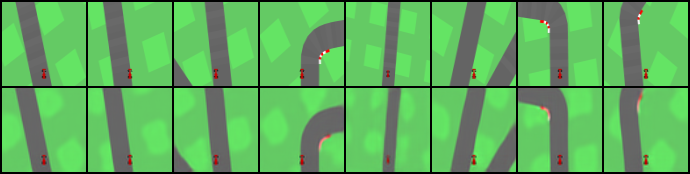
\includegraphics[width=0.92\textwidth]{VQVAE/80.png}

  \medskip
  {\footnotesize Topo: frame original \quad$\vert$\quad Base: reconstrução do VQ-VAE
  (após 400 épocas). A geometria da pista e a posição do carro são
  preservadas com fidelidade.}

  \vfill
  {\scriptsize\textcolor{gray}{Treino: MSE + VQ commitment \textperiodcentered{} AdamW (lr $10^{-4}$) \textperiodcentered{}
  batch 128 \textperiodcentered{} 400 épocas \textperiodcentered{} AMP \textperiodcentered{} grad clip 1.0}}
\end{frame}

\begin{frame}{VQ-VAE --- Uso do Codebook}
  \begin{columns}[c]
    \begin{column}{0.6\textwidth}
      \centering
      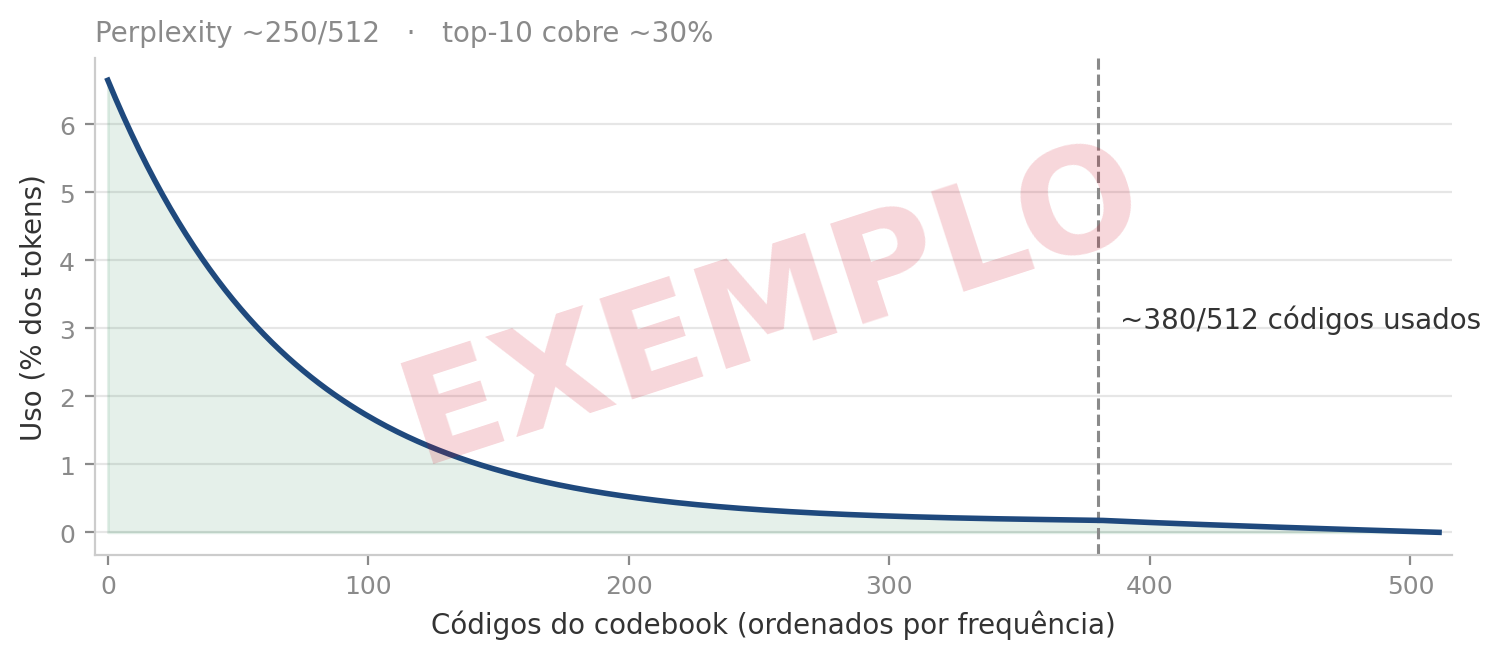
\includegraphics[width=\textwidth]{slides_assets/codebook_usage.png}
    \end{column}
    \begin{column}{0.38\textwidth}
      \small
      \begin{block}{Por que medir?}
        \footnotesize
        Um codebook saudável usa \textbf{muitos dos 512 códigos} e evita
        \emph{codebook collapse} (poucos códigos dominando). Métricas:
        \begin{itemize}
          \item códigos ativos / 512
          \item \textbf{perplexity} $=e^{H(p)}$
          \item \% coberto pelo top-10
        \end{itemize}
      \end{block}
    \end{column}
  \end{columns}

  \smallskip
  {\scriptsize\textcolor{red!70!black}{\textbf{Figura ilustrativa (EXEMPLO).}}
  \textcolor{gray}{Gerar os números reais com
  \texttt{results/plot\_codebook\_usage.py} sobre o dataset tokenizado / VQ-VAE
  treinado, e recompilar.}}
\end{frame}

% =====================================================================
\section{Modelo de Dinâmica --- GPT}

\begin{frame}{GPT Dynamics --- Layout de Sequência}
  \small\texttt{models/dynamics/gptimage.py}, \texttt{trainimage.py}
  \medskip

  O modelo prevê os \textbf{64 tokens} do próximo frame dado um contexto de
  \textbf{19 frames} + a ação a executar. Cada frame é um \emph{bloco de 65
  tokens}:
  \medskip

  \[
    \underbrace{z_0,\; z_1,\; \ldots,\; z_{63}}_{64\text{ tokens visuais}},\;
    \underbrace{a}_{1\text{ ação}}
  \]

  \medskip
  \begin{block}{Dimensões}
    \begin{itemize}
      \item Sequência de entrada: $19 \times 65 = \mathbf{1235}$ tokens.
      \item \texttt{block\_size} máximo: $20 \times 65 = \mathbf{1300}$
            (contexto + bloco alvo).
    \end{itemize}
  \end{block}
\end{frame}

\begin{frame}{GPT Dynamics --- Como o Transformer prevê}
  \centering
  \resizebox{0.97\textwidth}{!}{%
  \begin{tikzpicture}[x=1cm,y=1cm, every node/.style={font=\scriptsize}]
    % stream de tokens: blocos de frame
    \node[draw=acc2, thick, fill=acc!18, minimum height=0.7cm, minimum width=1.7cm] (f1) at (0,0) {$z_0\!\ldots z_{63}$};
    \node[draw=acc2, thick, fill=acc2!25, minimum height=0.7cm, minimum width=0.6cm, right=0pt of f1] {$a$};
    \node at (2.9,0) {$\cdots$};
    \node[draw=acc2, thick, fill=acc!18, minimum height=0.7cm, minimum width=1.7cm] (f2) at (4.6,0) {$z_0\!\ldots z_{63}$};
    \node[draw=acc2, thick, fill=acc2!25, minimum height=0.7cm, minimum width=0.6cm, right=0pt of f2] (a2) {$a$};
    \node[lbl] at (2.3,-0.75) {19 frames de contexto ($19{\times}65=1235$ tokens)};

    % embeddings
    \node[align=center] (emb) at (2.6,-1.9) {\,obs\_emb$(512{\to}256)$ + act\_emb$(5{\to}256)$ + pos\_emb\,};
    \draw[ar] (2.6,-0.4) -- (emb);

    % transformer stack
    \node[draw=acc2, very thick, rounded corners, fill=acc2!10, minimum width=6cm, minimum height=1.2cm, align=center]
      (tr) at (2.6,-3.4) {\textbf{Transformer causal} --- 6 camadas $\times$ (4 cabeças + MLP $d_{ff}{=}1024$)\\ \scriptsize máscara triangular: token $t$ só vê $\le t$};
    \draw[ar] (emb) -- (tr);

    % head + prediction
    \node[draw=acc2, thick, fill=acc!30, minimum height=0.7cm, minimum width=2.4cm, align=center] (pred) at (9.6,-3.4)
      {cabeça $256{\to}512$\\\scriptsize softmax por token};
    \draw[ar] (tr) -- (pred);
    \node[draw=acc2, thick, fill=acc!18, minimum height=0.7cm, minimum width=2.0cm] (nf) at (9.6,-1.0) {$\hat z_0\!\ldots\hat z_{63}$};
    \node[lbl] at (9.6,-0.25) {frame $t{+}1$ (64 tokens)};
    \draw[ar] (pred) -- (nf);

    % causal mask mini
    \node[lbl] at (6.2,-4.4) {cross-entropy vs.\ tokens reais (teacher forcing)};
  \end{tikzpicture}}

  \medskip
  {\footnotesize O modelo é um \textbf{GPT}: prediz o próximo token do stream. Ao prever os
  64 tokens do frame seguinte condiciona-se no contexto \emph{e} na ação $a$.}
\end{frame}

\begin{frame}{GPT Dynamics --- Arquitetura e Treino}
  \begin{columns}[T]
    \begin{column}{0.52\textwidth}
      \textbf{Arquitetura}
      \footnotesize
      \begin{table}
        \begin{tabular}{ll}
          \toprule
          Componente & Detalhe \\
          \midrule
          \texttt{obs\_emb} & $512 \to 256$ (amarrado à cabeça) \\
          \texttt{act\_emb} & $5 \to 256$ \\
          \texttt{pos\_emb} & aprendido, 1300 pos. \\
          Transformer & 6 cam., 4 cab., $d_{ff}{=}1024$ \\
                       & GELU, \texttt{norm\_first} \\
          Máscara & causal (triangular) \\
          Cabeça & $256 \to 512$ (tied) \\
          \bottomrule
        \end{tabular}
      \end{table}
      {\scriptsize$\sim$4\,M de parâmetros}
    \end{column}
    \begin{column}{0.46\textwidth}
      \textbf{Treinamento}
      \footnotesize
      \begin{table}
        \begin{tabular}{ll}
          \toprule
          Hiperparâm. & Valor \\
          \midrule
          Loss & cross-entropy (token) \\
          Otimizador & AdamW, wd $0.01$ \\
          lr & $10^{-4}$ \\
          Batch & 32 \\
          Épocas & 5000 \\
          Precisão & AMP \\
          Grad clip & 1.0 \\
          Contexto & 19 frames \\
          \bottomrule
        \end{tabular}
      \end{table}
      \smallskip
      {\scriptsize\textbf{Teacher forcing}: concatena o frame alvo ao contexto
      e prevê cada token com shift de posição no bloco.}
    \end{column}
  \end{columns}
\end{frame}

\begin{frame}{GPT Dynamics --- Inferência Autorregressiva}
  \small\texttt{imagine\_next\_frame}
  \medskip

  \begin{itemize}
    \item Os 64 tokens do próximo frame são gerados \textbf{um a um}.
    \item \textbf{Top-$k$ sampling} ($k=50$, temperatura $=1.0$) --- evita tokens
          de baixíssima probabilidade sem colapsar para \emph{greedy}.
    \item \textbf{Janela deslizante}: a cada frame gerado, descarta-se o mais
          antigo e insere-se o recém-criado, mantendo sempre 19 frames de
          contexto.
  \end{itemize}

  \bigskip
  \centering
  \begin{tikzpicture}[node distance=0.4cm]
    \node[stg, text width=2.6cm] (ctx) {Contexto\\19 frames};
    \node[stg, text width=2.6cm, right=1.2cm of ctx] (gen) {Gera 64 tokens\\(top-$k$)};
    \node[stg, text width=2.6cm, right=1.2cm of gen] (slide) {Desliza janela\\$+1$ frame};
    \draw[ar] (ctx) -- (gen);
    \draw[ar] (gen) -- (slide);
    \draw[ar] (slide.south) -- ++(0,-0.5) -| (ctx.south);
  \end{tikzpicture}
\end{frame}

% =====================================================================
\section{Resultados}

\begin{frame}{Resultados --- Sonho vs.\ Real}
  \small\texttt{models/dynamics/inferimage.py}
  \smallskip

  Seed de \textbf{19 frames} reais $\to$ modelo ``sonha'' \textbf{40 frames}
  usando as ações reais do episódio.

  \medskip
  \centering
  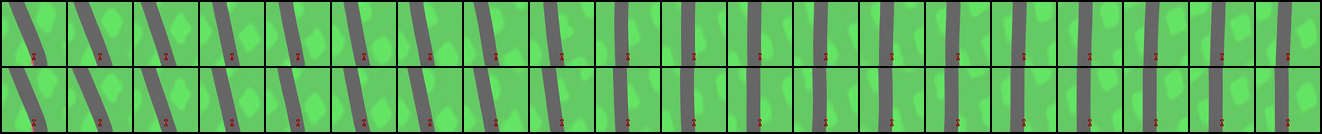
\includegraphics[width=\textwidth]{dreams/comparison.png}

  \smallskip
  {\footnotesize Linha superior: \textbf{sonho} do modelo \quad$\vert$\quad
  Linha inferior: \textbf{trajetória real}.}
\end{frame}

\begin{frame}{Resultados --- Rollout Sonhado (frames dos GIFs)}
  \centering
  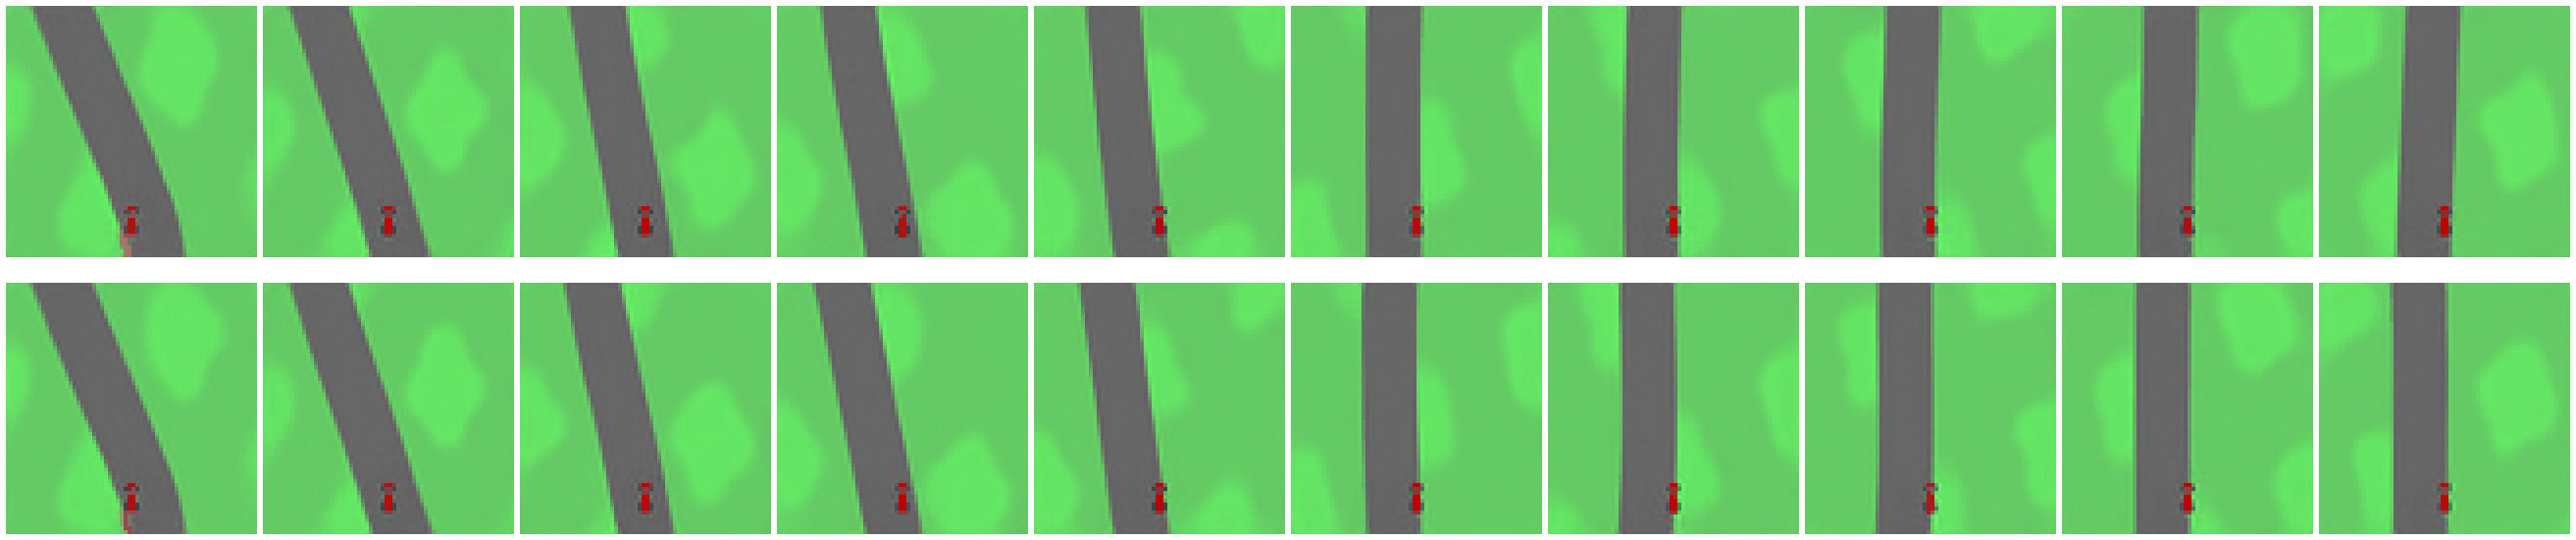
\includegraphics[width=\textwidth]{slides_assets/dream_vs_real_strip.png}

  \smallskip
  {\footnotesize Topo: \textbf{sonho} do modelo (rollout autorregressivo) \quad$\vert$\quad
  Base: \textbf{real}. Frames amostrados de \texttt{dream\_from\_grid.gif} /
  \texttt{real\_from\_grid.gif}.}

  \vfill
  {\scriptsize\textcolor{gray}{GIFs animados disponíveis em \texttt{results/dreams/} e
  frames individuais em \texttt{results/slides\_assets/}.}}
\end{frame}

\begin{frame}{Resultados --- Degradação Quantitativa}
  \begin{columns}[c]
    \begin{column}{0.62\textwidth}
      \centering
      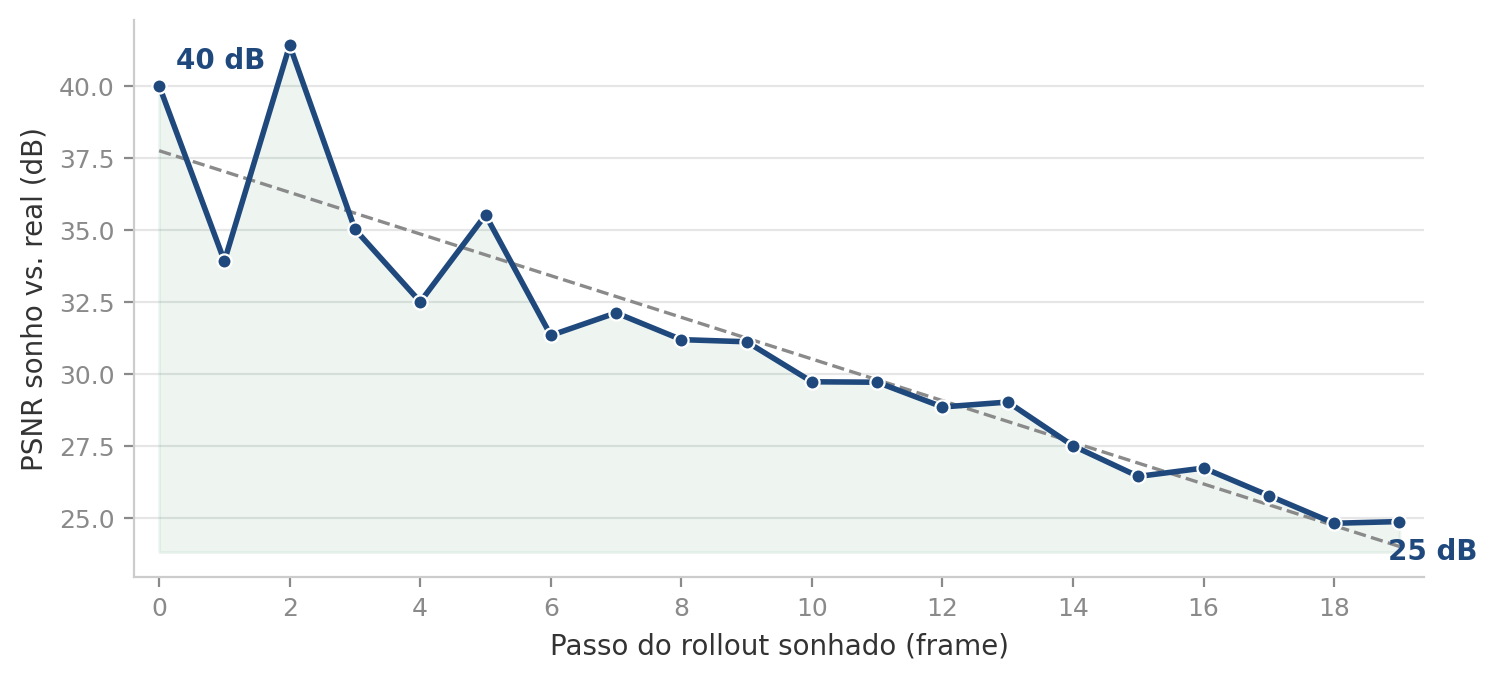
\includegraphics[width=\textwidth]{slides_assets/psnr_curve.png}
    \end{column}
    \begin{column}{0.36\textwidth}
      \footnotesize
      \begin{table}
        \begin{tabular}{@{}ll@{}}
          \toprule
          Métrica (rollout 20f) & Valor \\
          \midrule
          PSNR inicial (f.\,0)  & $40{,}0$ dB \\
          PSNR final (f.\,19)   & $24{,}9$ dB \\
          PSNR médio            & $30{,}9$ dB \\
          Queda por frame       & $-0{,}72$ dB \\
          \bottomrule
        \end{tabular}
      \end{table}
      \smallskip
      {\scriptsize O sonho parte quase idêntico ao real e \textbf{diverge de forma
      suave e monótona} --- coerente com a inspeção visual da filmstrip.}
    \end{column}
  \end{columns}

  \smallskip
  {\scriptsize\textcolor{gray}{PSNR calculado frame-a-frame entre
  \texttt{dream\_from\_grid.gif} e \texttt{real\_from\_grid.gif}.}}
\end{frame}

\begin{frame}{Resultados --- Análise}
  \begin{block}{Observações qualitativas}
    O modelo mantém a \textbf{estrutura global da pista} --- geometria da curva,
    posição do carro, coloração do gramado --- ao longo dos frames sonhados,
    com \emph{degradação gradual} dos detalhes finos à medida que a predição
    se afasta do seed.
  \end{block}

  \bigskip
  \begin{block}{Sanidade quantitativa}
    \textbf{Token accuracy} --- fração dos 64 tokens sonhados que coincidem
    exatamente com os reais --- é reportada ao fim de cada execução da
    inferência.
  \end{block}

  \bigskip
  \small Saídas geradas: \texttt{dream.gif} (sonho), \texttt{real.gif} (real)
  e \texttt{comparison.png} (grid comparativo).
\end{frame}

% =====================================================================
\section{Escolhas de Design}

\begin{frame}{Resumo das Escolhas de Design}
  \small
  \begin{table}
    \begin{tabular}{@{}p{4.3cm} p{7.6cm}@{}}
      \toprule
      \textbf{Decisão} & \textbf{Motivação} \\
      \midrule
      Discretização VQ-VAE &
        Tokens simplificam a previsão do GPT (cross-entropy vs.\ regressão). \\[3pt]
      Atenção só em baixa resolução &
        Reduz custo quadrático mantendo capacidade global ($8{\times}8$, $16{\times}16$). \\[3pt]
      Pesos amarrados (tied) &
        Regularização padrão; reduz parâmetros sem perder expressividade. \\[3pt]
      $\varepsilon$-schedule crescente &
        Cobre estados raros sem sacrificar a qualidade média do dataset. \\[3pt]
      Teacher forcing &
        Estabilidade de gradiente; evita BPTT longo. \\[3pt]
      Top-$k$ sampling &
        Evita tokens improváveis sem colapsar para greedy. \\
      \bottomrule
    \end{tabular}
  \end{table}
\end{frame}

% =====================================================================
\section{Passos Futuros}

\begin{frame}{Passos Futuros}
  \begin{block}{Modelo de dinâmica completo}
    \begin{itemize}
      \item Prever também \textbf{recompensa} e \textbf{done} por frame
            (já disponíveis no dataset) --- fechar o world model como MDP.
      \item Estender o horizonte de sonho e medir \emph{drift} acumulado.
    \end{itemize}
  \end{block}

  \begin{block}{Aprendizado no ``sonho''}
    \begin{itemize}
      \item Treinar um \textbf{controlador} inteiramente dentro do world model
            (à la Ha \& Schmidhuber) e transferir para o ambiente real.
      \item Avaliar \emph{return} da política aprendida no sonho vs.\ no jogo.
    \end{itemize}
  \end{block}

  \begin{block}{Avaliação e escala}
    \begin{itemize}
      \item Métricas de fidelidade perceptual (LPIPS, FID) além de token accuracy.
      \item Escalar contexto / parâmetros do GPT e refinar o codebook do VQ-VAE.
    \end{itemize}
  \end{block}
\end{frame}

\begin{frame}{Passos Futuros --- O Ciclo do World Model}
  \centering
  \resizebox{0.80\textwidth}{!}{%
  \begin{tikzpicture}[x=1cm,y=1cm, node distance=5.2cm]
    % --- nós principais do loop imaginado ---
    \node[stg, fill=acc!18, text width=3.2cm, minimum height=1.6cm] (ag)
      {\textbf{Agente} / Controlador\\\scriptsize política $\pi(a\mid z)$};
    \node[stg, right=of ag, text width=3.4cm, minimum height=1.6cm] (wm)
      {\textbf{World Model}\\\scriptsize VQ-VAE + GPT\\(sonho, sem o jogo)};

    % --- loop: ação -> world model ; estado/recompensa -> agente ---
    \draw[ar, bend left=22] (ag) to
      node[above, font=\scriptsize, align=center]{ação $a_t$} (wm);
    \draw[ar, bend left=22] (wm) to
      node[below, font=\scriptsize, align=center]{$z_{t+1}$,\; $\hat r_t$,\; $\widehat{\text{done}}_t$} (ag);

    % --- sinal de aprendizado ---
    \node[op, above=0.6cm of ag, fill=acc!20] (rl) {RL};
    \draw[ar, dashed] (wm.north) to[bend right=18]
      node[above, font=\scriptsize]{maximiza $\sum \hat r_t$} (rl);
    \draw[ar, dashed] (rl) -- (ag.north);

    % --- visualização opcional via decoder ---
    \node[stg, below=1.6cm of wm, text width=3.0cm, minimum height=0.9cm, fill=acc2!12] (dec)
      {\scriptsize Decoder $\to$ frame (visual)};
    \draw[ar, densely dotted] (wm) -- (dec);

    % --- transferência para o ambiente real ---
    \node[stg, below=1.6cm of ag, text width=3.2cm, minimum height=1.2cm, fill=gray!12, draw=gray!60] (env)
      {\textbf{Ambiente real}\\\scriptsize \texttt{CarRacing-v3}\\(só avaliação)};
    \draw[ar, thick, draw=acc] (ag) --
      node[left, font=\scriptsize, align=center]{transfere\\política} (env);
    \draw[ar, densely dashed, draw=gray!60] (env) to[bend left=25]
      node[below, font=\scriptsize]{\emph{return} real} (rl);
  \end{tikzpicture}}

  \smallskip
  {\footnotesize O agente é treinado \textbf{inteiramente dentro do sonho} --- sem rodar o
  jogo --- e só usa o \texttt{CarRacing} real para \emph{avaliar} a política transferida
  (à la Ha \& Schmidhuber, 2018).}
\end{frame}

% =====================================================================
\section{Demo}

\begin{frame}{Demo --- Rollout Animado (Sonho vs. Real)}
  \centering
  % GIF embutido como sequência de frames (f0..f19). Toca no Adobe Acrobat/Reader.
  % autoplay+loop+controls; 5 fps -> ~4 s por volta.
  \animategraphics[autoplay,loop,controls,height=0.56\textheight]%
    {5}{slides_assets/anim/f}{0}{19}

  \smallskip
  {\footnotesize A anima\c{c}\~ao roda no \textbf{Adobe Acrobat/Reader} (ou \texttt{pdfpc});
  em outros leitores aparece o primeiro frame.\;
  \textcolor{gray}{Link opcional:
  \href{https://SEU-LINK-AQUI}{\texttt{https://SEU-LINK-AQUI}}}}
\end{frame}

% =====================================================================
\begin{frame}[plain]
  \centering
  \vfill
  {\LARGE\bfseries Obrigado!}\\[8pt]
  {\large Mundos Imaginados --- VQ-VAE + GPT Dynamics}\\[4pt]
  \textcolor{gray}{Lucas Barcelos}
  \vfill
\end{frame}

\end{document}
